%% abstrakte simplizialkomplexe

\section{Abstrakte Simplizialkomplexe}

Für topologische Anwendungen ist der $\R^N$ in vielen Fällen zu konkret
und unnötiger gedanklicher Balast. Deshalb sollte man die
Simplizialkomplexe unabhängig vom euklidischen Raum definieren. Diese
abstrakten Simplizialkomplexe werden in diesem Abschnitt
behandelt. Die zunächst stark erscheinende Vereinfachung stellt sich
als eine äquivalente Darstellung zu den geometrischen Komplexen
heraus.

\begin{Def}
  Eine nicht leere Menge $\Delta$ heißt \textbf{abstrakter
    Simplizialkomplex} oder auch nur abstrakter Komplex, falls mit
  jedem Element aus $\Delta$ auch jede Teilmenge aus diesem Element in
  $\Delta$ enthalten ist und jedes Element eine endliche Menge
  ist. Oder in Formeln geschrieben
  \renewcommand*{\theequation}{\textbullet}
  \begin{gather}
    \sigma \in \Delta \text{ und }  \tau \subset \sigma
    \Rightarrow \tau \in \Delta. \\
    \nonumber
    \forall \; \sigma \in \Delta : \sigma \text{ ist endliche Menge.}
  \end{gather}
  Für einen abstrakten Komplex werden folgende Begriffe benötigt:
  \begin{enumerate}[({A}1)]
% dimension, seite, knoten, unterkomplex, simpliziale abbildung, isomorphie
  \item Ein Element des Komplexes heißt \textbf{Simplex}. Die Teilmenge aller
    Simplexe der Mächtigkeit kleiner gleich $k$ heißt das \textbf{$k$-Skelett},
    insbesondere für $k=1$ ist dies die \textbf{Knotenmenge}.
  \item Die \textbf{Dimension} des Komplexes ist das Supremum über die
    Mächtigkeit der Seiten von $\Delta$. Für den leeren Komplex $\emptyset$ ist
    die Dimension $-1$.
  \item Eine Teilmenge vom Komplex, die (\textbullet) erfüllt, heißt
    \textbf{Unterkomplex}.
  \item Eine Abbildung zwischen den Knotenmengen zweier abstrakten
    Komplexe heißt \textbf{simpliziale Abbildung}, falls Seiten auf
    Seiten abgebildet werden.
  \item Zwei abstrakte Komplexe heißen \textbf{isomorph}, falls es eine
    bijektive simpliziale Abbildung gibt, deren Inverses auch
    simplizial ist.
  \item Sei $\Delta$ ein geometrischer Komplex, so bezeichnet die Menge
    \begin{gather*}
      V(\Delta) \coloneqq \set{ \sset{a_0 \ldots a_n} \subset
        \Delta^{(0)} }{ a_0 \ldots a_n \in \Delta}
    \end{gather*}
    das \textbf{Knotenschema} von $\Delta$.
  \item Ist ein abstrakter Komplex $\Delta$ isomorph zum Knotenschema
    eine geometrischen Komplexes $\Delta'$, so nennen wir $\Delta'$
    eine \textbf{geometrische Realisierung} von $\Delta$.
  \end{enumerate}
\end{Def}

\begin{Bsp}
  \begin{enumerate}[\textbullet]
  \item Für einen geometrischen Komplex $\sigma$ ist die Menge aller
    Knotenschemata zu jeder Seite von $\sigma$ ein abstrakter
    Simplizalkomplex und das Knotenschema wird auf triviale Art und
    Weise geometrisch durch $\sigma$ realisiert.
  \item Die Menge $\Delta = \sset{%
      \sset{a,b},\sset{a,c},%
      \sset{b,c},\sset{a},\sset{b},\sset{c},\emptyset}$
    ist ein abstrakter Komplex und seine geometrische Realisierung
    sieht wie folgt aus.
    \begin{center}
      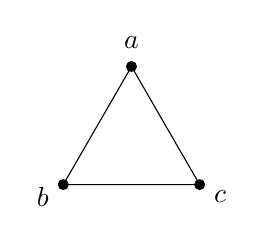
\begin{tikzpicture}
        \draw [thin] (90:1) to (210:1) to (330:1) to (90:1);
        \foreach \foo in {90,210,330}
        \fill (\foo:1) circle[radius=0.07cm];

        \node (a) at (90:1.3) {$a$};
        \node (b) at (210:1.3) {$b$};
        \node (c) at (330:1.3) {$c$};
      \end{tikzpicture}
    \end{center}

  \item Betrachte die Menge
    $\set{ \sset{i,i+1} , \sset{i} }{ i \in \Z} \cup \sset{\emptyset}$,
    dann ist der Polyeder zu einer geometrischen Realisierung
    homöomorph zu $\R$.

  \item Für eine Menge $M$, deren Elemente endliche Mengen sind, lässt
    sich stets ein abstrakter Komplex bilden, indem man alle
    Teilmengen der Elemente hinzu nimmt. Wir schreiben dies als
    $\pow^*(M)$.

  \item Die Von-Neumann-Zahlen liefern als Menge einen nicht endlichen
    abstrakten Komplex.  Diese Menge erhält man wie folgt. Definiere
    rekursiv $V_0 \coloneqq \emptyset$ und
    $V_{n+1} \coloneqq \sset{V_n} \cup \V_n$, dann ist
    $V \coloneqq \bigcup\limits_{n \geq 0} V_n$ ein nicht endlicher
    Komplex. Um einzusehen das die Menge wirklich einen abstrakten
    Komplex bildet sind nur die Regeln (\textbullet) nachzuweißen.
    Die unendliche Dimension ergibt sich daraus, dass man zu jeder
    natürlichen Zahl ein Element aus Komplex findet, das diese
    Dimension besitzt.
    
  \item Ein ungerichteter Graph $G=(V,K)$ mit $V$ die Eckmenge und $K$
    die Kanten ist ein abstrakter Simplizialkomplex.
  \item Das Knotenschema von einem geometrischen Komplex ist ein
    abstrakter Komplex.
  \end{enumerate}
\end{Bsp}

Der folgende Satz hat als Aussage, dass das letzte Beispiel das
Entscheidende ist. Der Zusammenhang zwischen geometrischen und
abstrakten Komplexen ergibt sich aus dem folgenden Satz.


\begin{Satz}
  Es gelten folgende Aussagen:
  \begin{enumerate}[(1)]
  \item Für jeden abstrakten Komplex existiert ein geometrischer
    Komplex, dessen Knotenschema (abstrakt) isomorph zu diesem Komplex
    ist.
  \item Zwei geometrische Komplexe sind (linear) isomorph, genau dann
    wenn die dazugehörigen Knotenschemata (abstrakt) isomorph sind.
  \end{enumerate}
  \begin{proof}
    \begin{enumerate}[(1)]
    \item Nach \cref{satz:geosimp} $(e)$ existiert für einen
      endlichen geometrischen Komplex stets ein Standardkomplex
      $\Delta^n$, sodass dieser als ein isomorpher Teilkomplex darin
      enthalten ist. Verallgemeinere nun diesen Standardkomplex auf
      einen unendlich dimensionalen im Raum $\E^J$. Hierzu wird
      $\Delta^J$ von all den Einheitsvektoren im $\E^J$
      aufgespannt. Dies bildet wiederum einen geometrischen Komplex.

      Sei nun ein abstrakter Komplex $\Delta$ und seine Knotenmenge
      $\Delta^{(0)}$ gegeben, dann betrachte die Einbettung
      $f : \Delta^{(0)} \rightarrow J$.  Es ist nun klar, dass die
      Simplexe, die von den Einheitsvektoren $e_j$ aus dem Bild von
      $f$ aufgespannt werden, einen geometrischen Komplex bilden, der
      nach Konstruktion ein Knotenschema besitzt, das isomorph zu
      $\Delta$ ist.

    \item Seien zwei geometrischen Komplexe $\Delta,\Delta'$ mit ihren
      Knotenschemata $V(\Delta),V(\Delta')$ gegeben. Falls nun ein
      Isomorphismus zwischen $\Delta,\Delta'$ existiert dann erfüllt
      er eingeschränkt auf die Knotenmenge genau die Eigenschaft der
      abstrakten simplizialen Abbildung zwischen den Knotenschemata
      als abstrakte Komplexe und somit entsprechen sich diese
      Isomorphismen gegenseitig.
    \end{enumerate}
  \end{proof}
\end{Satz}

% todo: topologie --literatur/archiv seite 333ff

% erkläre das labeln von triangulierungen, bzw
% geometrischen,abstrakten simplizialkomplexen

% \begin{Bem}[Label,Abwicklung]
%   Da im weiteren Verlauf des Seminars meist nicht zweidimensionale
%   Triangulierungen angegeben und benötigt werden, ist es notwendig,
%   eine vereinfachte Darstellung dieser höher dimensionalen Objekte
%   abzugeben. Hierzu wird das Labeln von Triangulierungen angegeben.

%   Betrachte zunächst für die Idee des Verfahrens den Tetraeder und
%   seine Standardabwicklung im Zweidimensionalen.
%   % zeichne dreidim tetraeder, und eine zweidim abwicklung, tikz
%   Bei der Abwicklung werden die $0$-Simplexe fortlaufend alphabetisch
%   nummeriert. Bei Knoten, die in der ursprünglichen Dimension
%   zusammenfallen wird das gleiche Label verwendet.

% %TODO: auch für unendlich dimensionale abwicklung
%   Die Formalisierung der obigen Idee wird durch die Angabe eines
%   abstrakten Komplexes gegeben, dessen geometrische Realisierung dem
%   geometrischen Komplex entspricht. Sei $\Delta$ ein endlich
%   dimensionaler geometrischer Komplex gegeben. Dann ist die Abwicklung
%   durch einen zweidimensionalen geometrischen Komplex $\Delta'$ und
%   eine surjektive Abbildung $f: \Delta \rightarrow \Delta'$ gegeben.

% %TODO: weiter ausführen

% \end{Bem}

% % TODO: label und zweidim abwicklungen vom torus, zylinder, kugel und kleinsche flasche

%einfache beispiele

\begin{Bsp}[Triangulierung]
  Es werden nun Triangulierungen für Sphäre, Zylinder und Torus
  angegeben durch abstrakte Komplexe, deren Geometrische Realisierungen
  eine Triangulierung der entsprechenden Flächen im $\R^3$ sind.

  \begin{description}
  \item[Zylinder:] Wir betrachten die Menge
    \begin{gather*}
      \Delta \coloneqq
      \sset{\sset{a,b,c},\sset{b,c,e},\sset{c,e,f},\sset{c,d,f}%
        ,\sset{a,d,f},\sset{a,b,f}}
    \end{gather*}
    Dann ist $\pow^*(\Delta)$ ein abstrakter Komplex.  Durch
    identifizieren der Punkte gleichen Labels wird durch
    zusammenfalten im dreidimensionalen daraus eine Fläche, die
    homöomorph zur Zylinderoberfläche ist. Dies sieht man unmittelbar
    ein, indem man zunächst annimmt, dass die Kante $\sset{a,b}$
    parallel zur $z$-Achse im $\R^3$ ist und dann eine
    Normierungsabbildung in der $x-y$-Ebene als Abbildung verwendet.
    \newline
  \begin{center}
      \parbox{0.7\linewidth}{%
      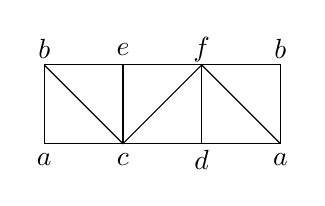
\begin{tikzpicture}
        \draw(0,0) rectangle (3,1); 
        \draw (1,0) to (1,1);
        \draw (2,0) to (2,1);
        \draw (0,1) to (1,0) to (2,1) to (3,0);

        \node (a1) at (0,-0.2) {$a$};
        \node (c) at (1,-0.2) {$c$};
        \node (d) at (2,-0.2) {$d$};
        \node (a2) at (3,-0.2) {$a$};

        \node (b1) at (0,1.2) {$b$};
        \node (e) at (1,1.2) {$e$};
        \node (f) at (2,1.2) {$f$};
        \node (b2) at (3,1.2) {$b$};
      \end{tikzpicture}
      \hfill
      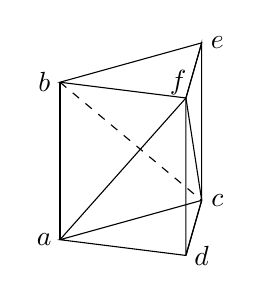
\begin{tikzpicture}
        \node (a) at (-0.2,0.2) {$a$};
        \node (b) at (-0.2,2.2) {$b$};
        \node (c) at (2,0.7) {$c$};
        \node (d) at (1.8,0) {$d$};
        \node (e) at (2,2.7) {$e$};
        \node (f) at (1.5,2.2) {$f$};
%        \draw [thin,fill=lightgray] (0,0.2) to (1.8,0) to (1,1.7) to (0,0.2);
%        \draw [thin,fill=lightgray] (1.8,0) to (1.8,0.7) to (1,1.7) to (1.8,0);
%        \draw [thin,dashed] (1.8,0.7) to (0,0.2);
        \draw [thin] (1.6,0) to (1.8,0.7) to (0,0.2) to (1.6,0);
        \draw [thin] (1.6,2) to (1.8,2.7) to (0,2.2) to (1.6,2);
        \draw [thin] (1.6,0) to (1.8,0.7) to (1.8,2.7) to (1.6,2) to (1.6,0);
        \draw [thin] (0,0.2) to (0,2.2);
        \draw [thin,dashed] (0,2.2) to (1.8,0.7);
        \draw [thin] (1.8,0.7) to (1.6,2);
        \draw [thin] (1.6,2) to (0,0.2);
      \end{tikzpicture}}
    \end{center}
  \item[Torus:] Zur Triangulierung des Torus ($\Sp^1 \times \Sp^1$)
    ist ein wesentlich komplizierterer abstrakter Komplex
    vonnöten.

    Betrachte hierzu die Menge
    \begin{align*}
      \Delta &\coloneqq \{ \sset{a,c,i},\sset{a,d,i},\\
        &\sset{b,c,f},\sset{c,f,i},\sset{a,b,d},\sset{b,d,f},\\
        &\sset{d,h,i},\sset{d,e,h},\sset{i,g,h},\sset{i,g,f},\\
        &\sset{d,e,f},\sset{e,f,g},\sset{a,c,e},\sset{c,e,h},\\
        &\sset{b,c,h},\sset{b,g,h},\sset{a,b,g},\sset{a,e,g} \}
    \end{align*}

    Dann ist $\pow^*(\Delta)$ ein abstrakter Komplex.

    \begin{center}
    \parbox{0.8\linewidth}{%
      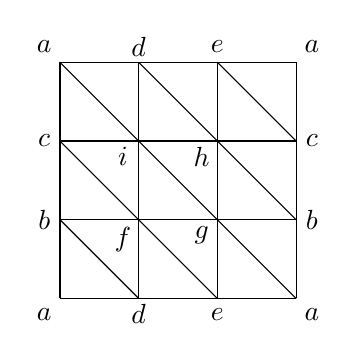
\begin{tikzpicture}
      \draw[step=1] (0,0)grid(3,3);    
      \draw [thin] (0,3) to (3,0);
      \draw [thin] (0,2) to (2,0);
      \draw [thin] (0,1) to (1,0);
      \draw [thin] (1,3) to (3,1);
      \draw [thin] (2,3) to (3,2);

        \node (a1) at (-0.2,-0.2) {$a$};
        \node (a2) at (3.2,-0.2) {$a$};
        \node (a3) at (3.2,3.2) {$a$};
        \node (a4) at (-0.2,3.2) {$a$};

        \node (b1) at (-0.2,1) {$b$};
        \node (b2) at (3.2,1) {$b$};
        \node (c1) at (-0.2,2) {$c$};
        \node (c2) at (3.2,2) {$c$};

        \node (d1) at (1,-0.2) {$d$};
        \node (d2) at (1,3.2) {$d$};
        \node (e1) at (2,-0.2) {$e$};
        \node (e2) at (2,3.2) {$e$};

        \node (f) at (0.8,0.75) {$f$};
        \node (g) at (1.8,0.8) {$g$};
        \node (h) at (1.8,1.8) {$h$};
        \node (i) at (0.8,1.8) {$i$};

    \end{tikzpicture}
    \hfill
    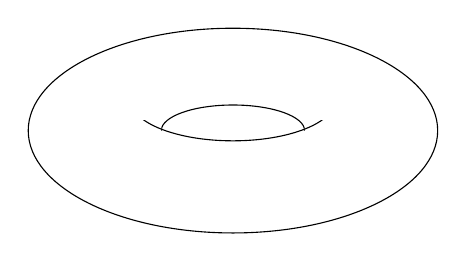
\begin{tikzpicture}[scale=1.3]
      \draw ellipse (2cm and 1cm);
      \begin{scope}
        \clip (-0.7,0)rectangle(0.7,0.5);
        \draw ellipse (0.7cm and 0.25cm);
      \end{scope}
      \begin{scope}
        \clip (-0.9,0.1)rectangle(0.9,-0.5);
        \draw (0,0.3) ellipse (1cm and 0.4cm);
      \end{scope}
    \end{tikzpicture}}
  \end{center}
  Identifiziert man nun jeweils die gegenüberliegende Seiten, indem
  man diese Seiten miteinander verklebt, erhält man den Torus als zwei
  dimensionale Fläche im $\R^3$.
\item[Sphäre:]
  Betrachte den Komplex
  \begin{gather*}
    \Delta \coloneqq \{ \sset{a,b,c},\sset{a,c,d},
    \sset{a,b,d},\sset{b,c,d} \}
  \end{gather*}
  und alle Teilmengen der Elemente oder kürzer geschrieben durch
  $\pow(\sset{a,b,c,d}) \setminus \{ a,b,c,d \}$.  Dann ist hierdurch
  eine Triangulierung der $\Sp^2$ gegeben.

  \begin{center}
    \parbox{0.7\linewidth}{%
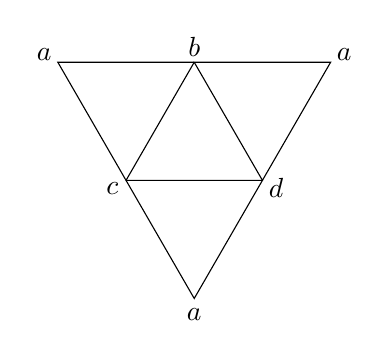
\begin{tikzpicture}
  \node (a1) at (30:2.2) {$a$};
   \node (a2) at (150:2.2) {$a$};
   \node (a3) at (270:2.2) {$a$};
   \node (b) at (90:1.2) {$b$};
   \node (c) at (210:1.2) {$c$};
   \node (e) at (330:1.2) {$d$};

%  \draw [thin] (90:1) to (210:1) to (330:1) to (90:1);
  \draw [thin] (330:1) to (30:2) to (90:1) to (330:1);
  \draw [thin] (90:1) to (150:2) to (210:1) to (90:1);
  \draw [thin] (210:1) to (270:2) to (330:1) to (210:1);
\end{tikzpicture}
\hfill
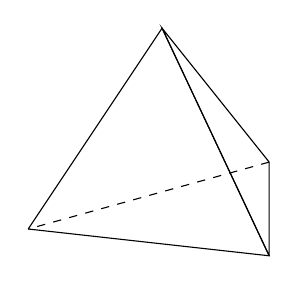
\begin{tikzpicture}[scale=1.7]
  \draw [thin] (0,1.2) to (1.8,1) to (1,2.7) to (0,1.2);
  \draw [thin] (1.8,1) to (1.8,1.7) to (1,2.7) to (1.8,1);
  \draw [thin,dashed] (1.8,1.7) to (0,1.2);
\end{tikzpicture}}
\end{center}

Beschreibt man nun diesen erhaltenen Tetraeder in eine Sphäre ein, so
folgt genauso wie in \cref{bsp:triangulierung}, dass dies eine
Triangulierung der Sphäre liefert.

\end{description}
  
\end{Bsp}

%TODO: beweise folgende triangulierengen \S^2 \simeq \gr{(\Delta^3)^{(2)}}, behauptung diese aussage gilt für allgemeines n, also \S^n \simeq \gr{(\Delta^{n+1})^{(n)}}





% abzählbare mengen können nur durch 0-simplexe trianguliert werden



%Begriffe:
%geometrisch unabhängig, und linear unabhängig vergleichen gegenüberstellen
% simplex, geometrischer simplizialkomplex, abstrakter simplizialkomplex 


% n-ebene, menge von punkten, aufgespannt durch geo.unab system mit konvexkombinationen
% die faktoren sind eindeutig bestimmt

%affine transformation: x -> Ax+b

%geo.unab systeme werden durch affine transformationen auf geo.unab systeme abgebildet

% n simplex

% baryzentrische koordinaten

% ist die leere menge eine simplizial?

% ein simplex ist genau die konvexe hülle von einer endlichen teilmenge vom \R^N

% eine seite eines simplex ist ein teilsimplex der dimension d

% anzahl der d teilsimplexe ist binomial_koeff(n+1,d+1), für einen n dim simplex
% klar wähle aus den n+1 punkten d+1 stück aus

% verwende das schläfli symbol zur beschreibung der umgebung eines
% punktes aus einem simplex für triangulierungen werden nur 2fache
% schläflisymbole benötigt, also {p,q}, da bei der triangulierung nur
% \laplace^2 simplexe verwendet werden, vereinfacht sich das symbol
% auf die form {3,q}. gebe nun zu jedem punkt auf der
% mannigfaltigkeit, also den 0 dimensionalen simplexen, die anzahl der
% angrenzenden dreiecker/laplace^2 simplexe an


% schreibe in die appendix ein eigenen anhang nur mit getikzten beispielen
% die komplette pflasterung von \R^2 oder allgemein die füllung des \R^n mit \laplace^n
% verschiedene triangulierungen

% zeige nicht-kompakte teilmengen vom \R^n sind nicht triangulierbar,
% einfachstes bsp (0,1), einfach das geometrische realisierungen stets
% kompakte mengen sind, somit kann es keinen homöomorphismus geben


%%% Local Variables:
%%% mode: latex
%%% TeX-master: "main"
%%% End: